\documentclass{standalone}
\usepackage{tikz}
\usepackage{ctex,siunitx}
\usepackage{tkz-euclide}
\usepackage{amsmath}
\usetikzlibrary{patterns, calc}
\usetikzlibrary {decorations.pathmorphing, decorations.pathreplacing, decorations.shapes,}
\begin{document}
\small
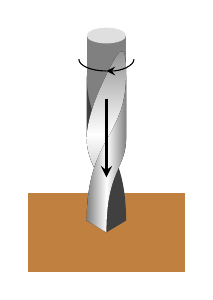
\begin{tikzpicture}[>=stealth]
  \fill [brown](-1,-1)rectangle(1,0);
  % \draw[thick](-1,0)--(1,0);
  \fill[gray](-0.25,2)rectangle(0.25,0.7);
  \fill[darkgray]
  (0,-0.5)--(0.25,-0.35)..controls(0.25,0.7)and(-0.25,0.7)..(-0.25,1.5)--(-0.25,0.7)..controls(-0.25,0.3)and(0,0.3)..(0,-0.5);
  \fill[top color=gray,bottom color=gray,middle color=white]
  (0,-0.5)..controls(0,0.3)and(-0.25,0.3)..(-0.25,0.7)..controls(-0.25,0.9)and(-0.15,1.2)..(0,1.5)..controls(0.15,1.8)and(0.25,2.0)..(0.25,1.5)--(0.25,0.7)--(0.05,0.7);
  \fill[left color=gray,right color=gray,middle color=white]
  (0.25,0.7)..controls(0.25,0.3)and(0,0.3)..(0,-0.5)--(-0.25,-0.35)..controls(-0.25,0.7)and(0.25,0.7)..(0.25,1.5)--cycle;
  \draw[thick,->](0,1.2)--++(0,-1);
  \fill[lightgray!50](0,2)ellipse(0.25 and 0.1);
  \draw(-0.35,1.7)arc(180:270:0.35 and 0.15);
  \draw[<-](0,1.55)arc(270:360:0.35 and 0.15);
\end{tikzpicture}
\end{document}